\documentclass[10pt]{article}
% see /usr/local/usrshare/share/doc/texlive-doc/latex/l2tabu-english/l2tabuen.pdf
%\usepackage{palatino}
\usepackage{mathpazo}
\usepackage[scaled=.95]{helvet}
\usepackage{courier}
\usepackage[l2tabu]{nag}
\usepackage{comment}
\input{vc.tex}
%%
% use this for draft!
%\usepackage[dark,landscape,timestamp]{draftcopy}
%\usepackage{pdfdraftcopy}
%\usepackage{verbatim}
%\usepackage{hyphenat}
%\usepackage{changebar}
%\usepackage[final]{pdfcomment}
%\usepackage{pdfcomment}
%\draftstring{DRAFT}
%\draftangle{45}
%\draftcolor{gray10}
% \RequirePackage{eso-pic,graphicx,color,type1cm}
% \AddToShipoutPicture{%
% \AtTextCenter{\makebox[0pt]{\scalebox{9}{%
%     \rotatebox[origin=c]{45}{\color[gray]{.8}\normalfont{Draft}}}}}} 
% not this \usepackage[final]{draftcopy}
%\usepackage{slashbox}
%\usepackage{xypic}
\usepackage{hyperref}
\usepackage{array}
\usepackage[pdftex]{graphicx}
\usepackage{tabularx}
\setlength{\extrarowheight}{3pt}
\newcommand*{\vcenteredhbox}[1]{\begingroup
\setbox0=\hbox{#1}\parbox{\wd0}{\box0}\endgroup}
\usepackage[none]{hyphenat}
%declare extensions
%\DeclareGraphicsExtensions{.jpg}
%\DeclareGraphicsRule{.jpeg}{eps}{.jpeg.bb}{`jpeg2ps #1}%
%\usepackage{pdflscape}
%\usepackage[pdftex]{lscape}
%\usepackage[landscape,pdftex]{geometry}
%\usepackage{lscape}
%\usepackage{rotating}
\usepackage{multirow}
%\usepackage{graphicx}
%\usepackage{html}
\usepackage{ifpdf}
%\usepackage{url}
\DeclareMathAlphabet{\mathscr}{OT1}{pzc}%
                                 {m}{it}
\setlength{\oddsidemargin}{-1cm}
\setlength{\topmargin}{-2.5cm}
\setlength{\textwidth}{27.5cm}
%\pdfoutput=0

\hyphenpenalty=1000\exhyphenpenalty=1000\relax
\sloppy%disable hyphenation
%\pdfpagewidth=297 mm % A4
%\pdfpageheight=210 mm
%\input{ps-draft}
  \def\Git$#1: #2 ${\expandafter\def\csname Git#1 \endcsname{#2}}
\begin{document}
%\setlength{\pdfpageheight}{\paperheight}
%\setlength{\pdfpagewidth}{\paperwidth}
\ifx\pdfoutput\undefined
\else
\pdfpagewidth=297 mm % A4
\pdfpageheight=210 mm
\fi
\begingroup
\ifpdf
%\pdfpageattr{/Rotate 90}
%\begin{landscape}
\else
\special{landscape}
\fi
\endgroup
\thispagestyle{empty}
%\DeclareGraphicsExtensions{.gif}
\begin{center}
%\caption{%{
{\Large 
%Draft
%
\includegraphics[width=1cm, scale=0.10]{bells.jpeg}
  AllSaints Rota 
%{\Huge Draft}
November -- December 2018
%
\includegraphics[width=1cm, scale=0.10]{bells.jpeg}
}%}
% \begin{figure}%[h]%t!]
%     \includegraphics{Koch-69a}
% \end{figure}
\vspace{0.5em}

% {\bf \Large \ldots for any final corrections - please check if dates are
%   impossible for you!} 
%\linebreak
%\rotatebox{90}{Advent}
%\begin{sloppypar}
{ \small
%% \begin{sidewaystable}[phbt]
% the 'P' column type is a ragged-right paragraph.  Uses array.sty
\newcolumntype{P}[1]{>{\raggedright}p{#1}}
\newcolumntype{X}[1]{>{\raggedright\arraybackslash}p{#1}}
\sloppy
\begin{tabular}{|%c | % Season
p{0.04\textwidth}| % Date
p{0.07\textwidth}| % Service
c| % Ldr
c| %Spkr
X{0.11\textwidth}| % Readings
X{0.07\textwidth}| % readers
p{0.06\textwidth}| % Prayers
X{0.08\textwidth}| %Side
% X{0.07\textwidth}| %Welc
X{0.09\textwidth}| % Tea
p{0.07\textwidth}| %Flwrs
p{0.06\textwidth}| % Breakfast creche
c|}\hline % collect sheets
%\begin{tabular}{|p{1.5cm}|p{1.8cm}|p{0.5cm}|p{0.5cm}|p{2.6cm}|p{2cm}|p{1.5cm}|p{2.4cm}|p{2.0cm}|p{2.2cm}
%\begin{tabular}{|p{1.6cm}|p{1.4cm}|p{0.6cm}|p{0.6cm}|p{2.8cm}|p{2cm}|p{1.5cm}|p{2.0cm}|p{2.0cm}|p{2.0cm}
%|p{1.8cm}|p{1.6cm}|}\hline
% heading
%{\bf
%& 
%\hline
 Date & Service & Leader & Spkr & Readings & Readers & Prayers &
Sidespersons & %Welcome Team &
 Tea &  Flowers & Breakfast  &{\footnotesize Printing} \\ \hline % & Cr\^{e}che
\hline
4 Nov & Informal & \multicolumn{2}{c|}{CC-K  DP } &  &  &  & Carol Fieldhouse Brian Gleaves   &  P Marsh S Ryder L Noonan A~Walton &  & Robert & JD \\ \hline
11 Nov & Holy Communion & KB & KB & Hebrews 9:24-28 Mark 1:14-20 & Ron Sherwin Chris Gleaves & Robert Marshall & Geoff \& Ann Walton & B \& C Gleaves E~Johnson & P Ashley & Chris and Brian & JD \\ \hline
18 Nov & Morning Worship & AW & CG & Mark 13:1-8 & Gillian Sly & Phil Marsh &  Richard Fieldhouse  Carol Fieldhouse & P \& S Gaskell C~Fieldhouse  & P Ashley & Margaret and Phil & PM \\ \hline
25 Nov & Holy Communion & JK & AW & Revelation 1:4b-8 John 18:33-37 & Phil Marsh Dot Phillips & Chris C-K & Sue Ryder Tony Hallatt & A Walton G Sly P~Marsh &  & Carol \& Richard & RS \\ \hline
2 Dec & Informal & \multicolumn{2}{c|}{CC-K/AC-P}   &  &  &  & Phil Marsh Ann Walton & L Hallatt D~\&~R~Graham R~Marshall  & P Gaskell \& P~Ashley & Ann \& Geoff & BG \\ \hline
9 Dec & Holy Communion & RW & RW & Philippians 1:3-11 Luke 3:1-6 & Linda Hallatt Joy Kewney  & Dot Graham & Sue Ryder Jim~Donaldson & S Ryder L~Noonan E~Johnson & Christmas Flowers & Jacqui & RM \\ \hline
16 Dec & Carol Service &  &  & \multicolumn{1}{c|}{Luke 3:7-18} & tba & tba & Geoff Walton Ron Sherwin & B \& C Gleaves  J~Donaldson & Christmas Flowers & Mike & JD \\ \hline
23 Dec & Holy Communion & AW & AW & Hebrews 10:5-10  Luke 1:39-45 & Carol Fieldhouse Tony Hallatt & Richard Fieldhouse & Chris C-K Ron~Sherwin & R Marshall G Sly C Fieldhouse & Christmas Flowers & Chris C-K & JD \\ \hline
24 Dec & Holy Communion & AW & AW & tba & Chris C-K Jacqui Donaldson & Chris Gleaves & Brian Gleaves Phil Marsh &  \multicolumn{4}{|c}{ \multirow{3}{*}{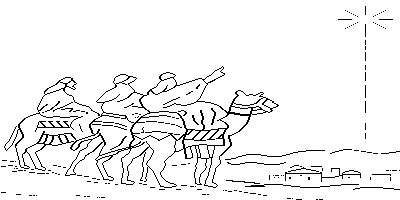
\includegraphics[width=3cm, scale=0.05]{christmas106}}}   \\ \cline{1-8} 
30 Dec & Team Service &  &  &  &  &  \multicolumn{4}{l}{}   \\ \hline
6 Jan & Informal & \multicolumn{2}{c|}{CC-K AC-P?}   & &  &  & Richard Fieldhouse Jim~Donaldson & P \& S Gaskell R~Marshall J~Donaldson & E Johnson & Pat \& Stephen & RM \\ \hline
\end{tabular}
\label{}
%\end{table}

\label{tab:LABEL} 
%\end{table}\end{tabular}
%\end{sidewaystable}
}
%\end{sloppypar}

\vspace{1em}
%% Books: \begin{tabular}{|l|l|} \hline
% Gen & Genesis &
% Ex & Exodus \\
% Deut & Deuteronomy &
% Is & Isaiah \\
% Zep & Zephaniah &
% Zech & Zechariah \\
% 1 Cor & 1 Corinthians &
%Rom & Romans \\
  % Eph & Ephesians &
% 2 Cor & 2 Corinthians &
%Phil & Philippians &
%Col & Colossians &
%% 1 Thess & 1 Thessalonians 
%% \\
%% %&
%%   \hline
%% \end{tabular}
%\begin{tabular}{|c|c|c|c|c|c|c|c|c|c|c|}\hline
\begin{comment}
\begin{tabular}{|c|c|c|c|}\hline
{\bf People: } & & & \\
%AAWT & All-Age Worship Team & %DW & David Wightman &
%% MT & Marion Tugwood \\
%GVT & Gerri Tetzlaff \\
%LS & Lynne Spedding \\
%BL+ & Bishop Libby &
%KB & Karen Brady \\
BL & Barry Langman &
MS & Magdalen Smith \\
%%JE & Jon Evans \\
%  GT & Graham Turner & RF & Richard Fieldhouse \\
%TH & Theresa Hayton & &  \\% JS & John Staley & 
%% IB & Ian Bishop &
%%  REM & Ruth Mock \\
%\\
%MS & Mike Strutt
%RW & Rob Wardle & & \\% & MH &  &  & \\
% VG & Vivien Gisby  & KR & Keith Ranger \\
% JG & Judith Gibson   &
% FH & Frances Hiles &
%& DM &  Dave Mock 
%AB & Andy Bull &
%KD & Kevin Dunn &
%PR & Philip Robinson &
%PS & Paul Spedding \\
% GT & Graham Turner &    %& JK & Joy Kewney   
%{\bf Abbreviations:}
%& nGP & No Godly Play 
%& tba & to be arranged \\
% {\bf Books: }  &  &   & 2 Cor & 2 Corinthians \\
%&   &  & 
%1 Thess & 1 Thessalonians & 
%\\ % & & & & & & & \\
%TG & Terry Gibson \\
% %FH & Frances Hiles & tba & to be arranged   \\ %\\ %JBu & John Buckley \\
% %BB & Barbara Bellfield & GC & Good Companions \\
% %  JM & John Mynett & MD & Mike Douglas \\
% % %  DW  & David Woodley & TG & Terry Gibson &%\\
% % %  RS & Ron Sutton & TS & Tony Sparham  \\
     \hline
\end{tabular}
\end{comment}
\end{center}
%\vspace{1em}
\hspace{1.15em}
\begin{minipage}{0.15\textwidth}
\ifpdf
%\begin{figure}%[hc]%t!]
%\hspace{2em}
%\fbox{
%\hspace{2em}
%\includegraphics[bb=0 0 75 70]{team1} Macclesfield Team Parish
%\vcenteredhbox{
\includegraphics[height=2.0cm, width=2.0cm]{newLogo}} Macclesfield Team Ministry
%}
%\end{figure}
\else
\hspace{0.5em}
%\includegraphics[bb=0 0 75 70]{team1} Macclesfield Team Parish
\fi
\end{minipage}
\begin{minipage}{0.75\textwidth}
%\begin{changebar} 
%{\bf 
{%}
%\end{changebar}
\footnotesize Please swap if you cannot do a date, see also list of names/tel nos.
Readers/Pray-ers -- if you swap, please let the service leader know.\\
 It would be helpful if sidespeople 
could arrive at 9.00am to ensure that service sheets and notice sheets are 
prepared and hymn numbers are put~up.
I aim to update the master copy with changes as they
happen and make it available -- for those with internet access
\linebreak -- at 
 \url{http://www.capuchin.co.uk/AS-rotas.html} 
%\url{http://brock-marshall.no-ip.info/~robert/AS-rotas}
(Robert Marshall 262151)}
\end{minipage}

\vspace{2em}
%Cr\^{e}che linked with 'Climbers' - contact Margaret Marsh
{\footnotesize 
%% Corrections to \url{&#109;&#97;&#105;&#108;&#116;&#111;&#58;&#114;&#111;&#98;&#101;&#114;&#116;&#64;&#99;&#97;&#112;&#117;&#99;&#104;&#105;&#110;&#46;&#99;&#111;&#46;&#117;&#107;}
%% \begin{htmlonly}
%% For corrections you can email me on the link at the foot of
%% \url{http://www.chezmarshall.freeserve.co.uk} (Robert Marshall)
%% a pdf form of the rota is available at
%% \url{http://brock-marshall.no-ip.info/~robert/AS-rotas/} - when my
%% home machine is booted!!

%% The reading listings are available at
%% \url{http://www.cofe.anglican.org/worship/liturgy/commonworship/resources/downloads/csvfile.html}
%% %http://www.cofe.anglican.org/commonworship/lect/lectfront1.html}.
%% Text of the readings can be found at
%% \url{http://divinity.library.vanderbilt.edu/lectionary/} - we are in Year B
%%  but the readings sometimes differ from the Anglican version!

%% %{\tiny  \$Id: AllSaintsRota.tex,v 1.62 2011/03/05 08:34:43 robert Exp $    }
%% %  \date{Revision \RCSRevision, \RCSDate}
%% %}

%% \end{htmlonly}
  Revision: \GITAbrHash \ % or any RCS keyword
  Date: \GITAuthorDate 
  %% \Git$Revision: 1.62 $ % or any RCS keyword
  %% \Git$Date: 2016/04/10 14:48:43 $

%{  \ $Id: AllSaintsRota.tex,v 1.62 2011/03/05 08:34:43 robert Exp $    }

%\begingroup
%\ifpdf
%\end{landscape}
%\fi
%\endgroup
}
\end{document}
